% Nallino, Part I p. 267: Schiaparelli's figure of the crescent of the Moon, redrawn from the print: the Moon L
% seen from T, the parallel lines TS and LS towards the Sun, the line TL through F, the diameter CD with the dark
% half hatched, the radius LB blank in the hatching, the radius LA, and the bold italic letters.
% Measured on the scan (_intake/latin/tools/fig267).
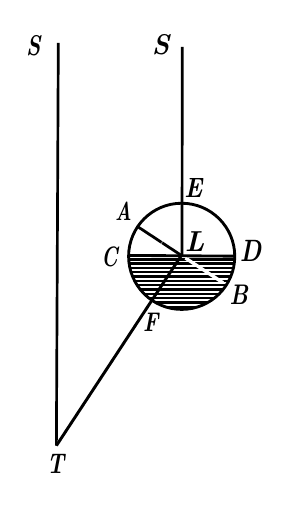
\begin{tikzpicture}[x=0.9964pt,y=-0.9964pt,line cap=butt,every node/.style={font=\fontsize{11}{11}\bfseries\itshape\selectfont,inner sep=0pt}]
\useasboundingbox (0,0) rectangle (86.00,163.00);
\begin{scope}\clip (55.85,82.92) circle[radius=19.25];
\clip (15.35,82.44) -- (96.35,83.01) -- (96.05,125.51) -- (15.05,124.94) -- cycle;
\draw[line width=0.84pt] (35.60,63.74) -- (76.10,63.74);
\draw[line width=0.84pt] (35.60,65.30) -- (76.10,65.30);
\draw[line width=0.84pt] (35.60,66.86) -- (76.10,66.86);
\draw[line width=0.84pt] (35.60,68.42) -- (76.10,68.42);
\draw[line width=0.84pt] (35.60,69.98) -- (76.10,69.98);
\draw[line width=0.84pt] (35.60,71.54) -- (76.10,71.54);
\draw[line width=0.84pt] (35.60,73.10) -- (76.10,73.10);
\draw[line width=0.84pt] (35.60,74.66) -- (76.10,74.66);
\draw[line width=0.84pt] (35.60,76.22) -- (76.10,76.22);
\draw[line width=0.84pt] (35.60,77.78) -- (76.10,77.78);
\draw[line width=0.84pt] (35.60,79.34) -- (76.10,79.34);
\draw[line width=0.84pt] (35.60,80.90) -- (76.10,80.90);
\draw[line width=0.84pt] (35.60,82.46) -- (76.10,82.46);
\draw[line width=0.84pt] (35.60,84.02) -- (76.10,84.02);
\draw[line width=0.84pt] (35.60,85.58) -- (76.10,85.58);
\draw[line width=0.84pt] (35.60,87.14) -- (76.10,87.14);
\draw[line width=0.84pt] (35.60,88.70) -- (76.10,88.70);
\draw[line width=0.84pt] (35.60,90.26) -- (76.10,90.26);
\draw[line width=0.84pt] (35.60,91.82) -- (76.10,91.82);
\draw[line width=0.84pt] (35.60,93.38) -- (76.10,93.38);
\draw[line width=0.84pt] (35.60,94.94) -- (76.10,94.94);
\draw[line width=0.84pt] (35.60,96.50) -- (76.10,96.50);
\draw[line width=0.84pt] (35.60,98.06) -- (76.10,98.06);
\draw[line width=0.84pt] (35.60,99.62) -- (76.10,99.62);
\draw[line width=0.84pt] (35.60,101.18) -- (76.10,101.18);
\end{scope}
\draw[line width=1.20pt,white] (57.22,83.55) -- (70.84,92.50);  % the radius LB, blank in the hatching
\draw[line width=1.03pt] (55.85,82.92) circle[radius=19.25];  % the Moon
\draw[line width=0.97pt] (10.41,151.57) -- (11.11,5.51);  % the line TS
\draw[line width=0.97pt] (55.96,82.73) -- (56.08,6.95);  % the line LE produced to S
\draw[line width=1.06pt] (10.41,151.57) -- (55.66,82.72);  % the line TL through F
\draw[line width=1.03pt] (36.60,82.59) -- (75.10,82.86);  % the diameter CD
% the radius LA, printed with a gap
\draw[line width=1.00pt] (55.96,82.73)--(48.78,78.01) (48.57,77.87)--(39.88,72.15);
\node at (2.02,6.58) {\normalfont\fontsize{11}{11}\bfseries\itshape\selectfont \resizebox{5.21pt}{7.07pt}{S}};
\node at (48.21,6.32) {\normalfont\fontsize{11}{11}\bfseries\itshape\selectfont \resizebox{6.36pt}{7.07pt}{S}};
\node at (60.08,58.18) {\normalfont\fontsize{11}{11}\bfseries\itshape\selectfont \resizebox{6.50pt}{6.93pt}{E}};
\node at (34.72,66.54) {\normalfont\fontsize{11}{11}\bfseries\itshape\selectfont \resizebox{5.99pt}{6.44pt}{A}};
\node at (60.54,77.70) {\normalfont\fontsize{11}{11}\bfseries\itshape\selectfont \resizebox{7.06pt}{7.16pt}{L}};
\node at (29.66,83.20) {\normalfont\fontsize{11}{11}\bfseries\itshape\selectfont \resizebox{5.92pt}{6.95pt}{C}};
\node at (80.80,80.94) {\normalfont\fontsize{11}{11}\bfseries\itshape\selectfont \resizebox{7.73pt}{7.65pt}{D}};
\node at (76.60,96.74) {\normalfont\fontsize{11}{11}\bfseries\itshape\selectfont \resizebox{6.66pt}{7.03pt}{B}};
\node at (44.64,106.66) {\normalfont\fontsize{11}{11}\bfseries\itshape\selectfont \resizebox{5.54pt}{6.69pt}{F}};
\node at (10.09,158.20) {\normalfont\fontsize{11}{11}\bfseries\itshape\selectfont \resizebox{6.29pt}{7.04pt}{T}};
\end{tikzpicture}
